\chapter{NDVI-MAP FUNCTIONS AND USER GUIDE}
\label{chap:ndvi & it's user guide}

\section{What can app do?}

Application can enable you to envision \gls{ndvi} mean information for any date accessible in the database. It likewise gives the usefulness of sending out the information into \gls{csv} record and messaging it to whosoever you need. \\
It likewise causes you visualize information utilizing diverse levels - Country wise, State wise and District.

\section{A user guide/manual}

\subsection{Getting Started}

\begin{itemize}
    \item \textbf{Downloading the app} \\ 
    \\
    Right now, the app is in process of being submitted to App Store for review. Once it is approved by Apple, you can utilize the "EyesOnCrops" application by downloading it from the Apple Store. 
    
    \begin{itemize}
        \item Open the App Store and type "EyesOnCrops" in search bar.
        \item Download and introduce the "EyesOnCrops" application on your gadget.
        \item Once the app is downloaded and installed, it will look like this on your device. You can have a look at Fig 2.1 for your reference.
        
        \begin{figure}[H]
            \centering
            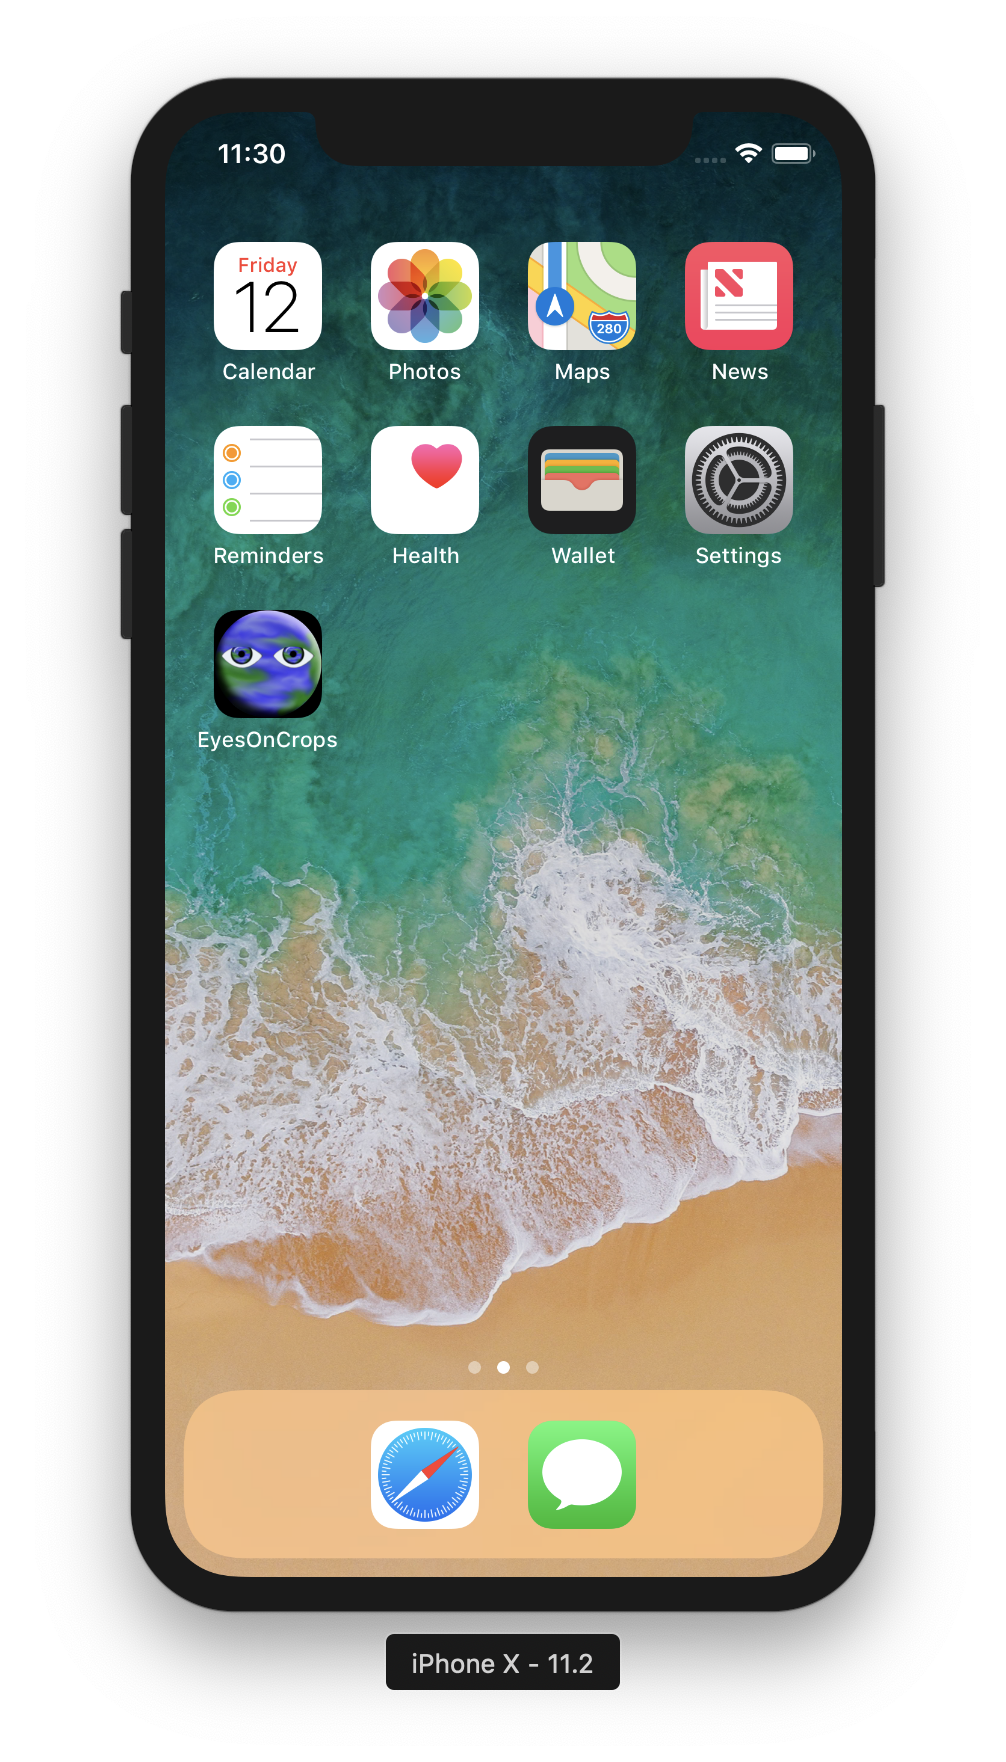
\includegraphics[width=0.5\linewidth]{figures/ch2/app_icon_screen.png}
            \caption{\label{fig:app_icon_screen} iPhone screen after downloading the app}
        \end{figure}
    \end{itemize}
    
    \item \textbf{Sign in} \\
    \\
    By tapping on app icon on fig 2.1, it will lake you to landing screen of the app which is also called as main screen.
    
     This screen gives you two options, which are (as shown in fig 2.2) :
     
       \begin{figure}[H]
            \centering
            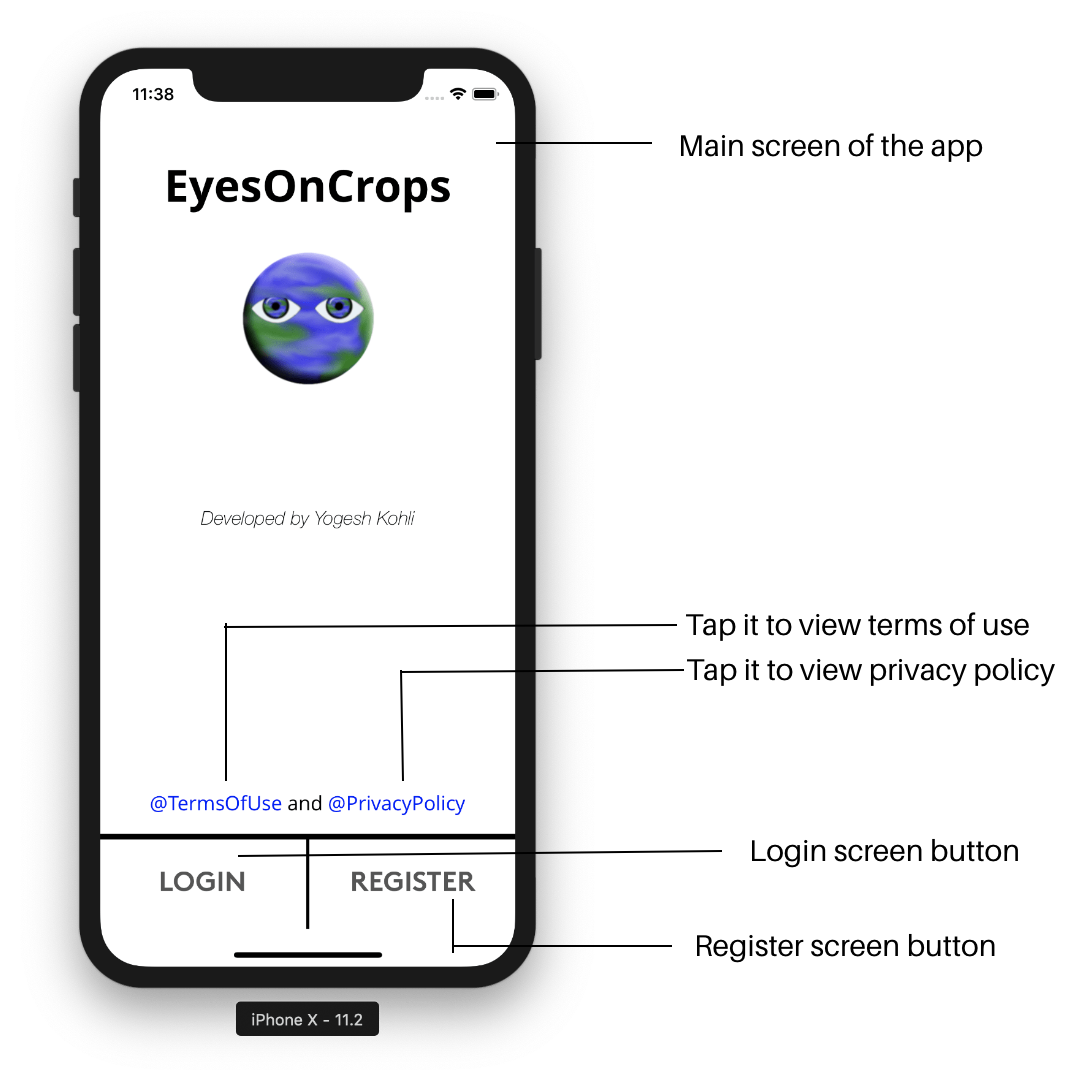
\includegraphics[width=0.5\linewidth]{figures/ch2/main_screen.png}
            \caption{\label{fig:main_screen} Main / Landing screen of the app}
        \end{figure}

    \textbf{1. Login} \\
    \textbf{2. Register via Email} \\
    
    If you select Login, it takes you two that screen which gives you options to enter the app. It has shown in fig 2.3.
    
    \begin{figure}[H]
            \centering
            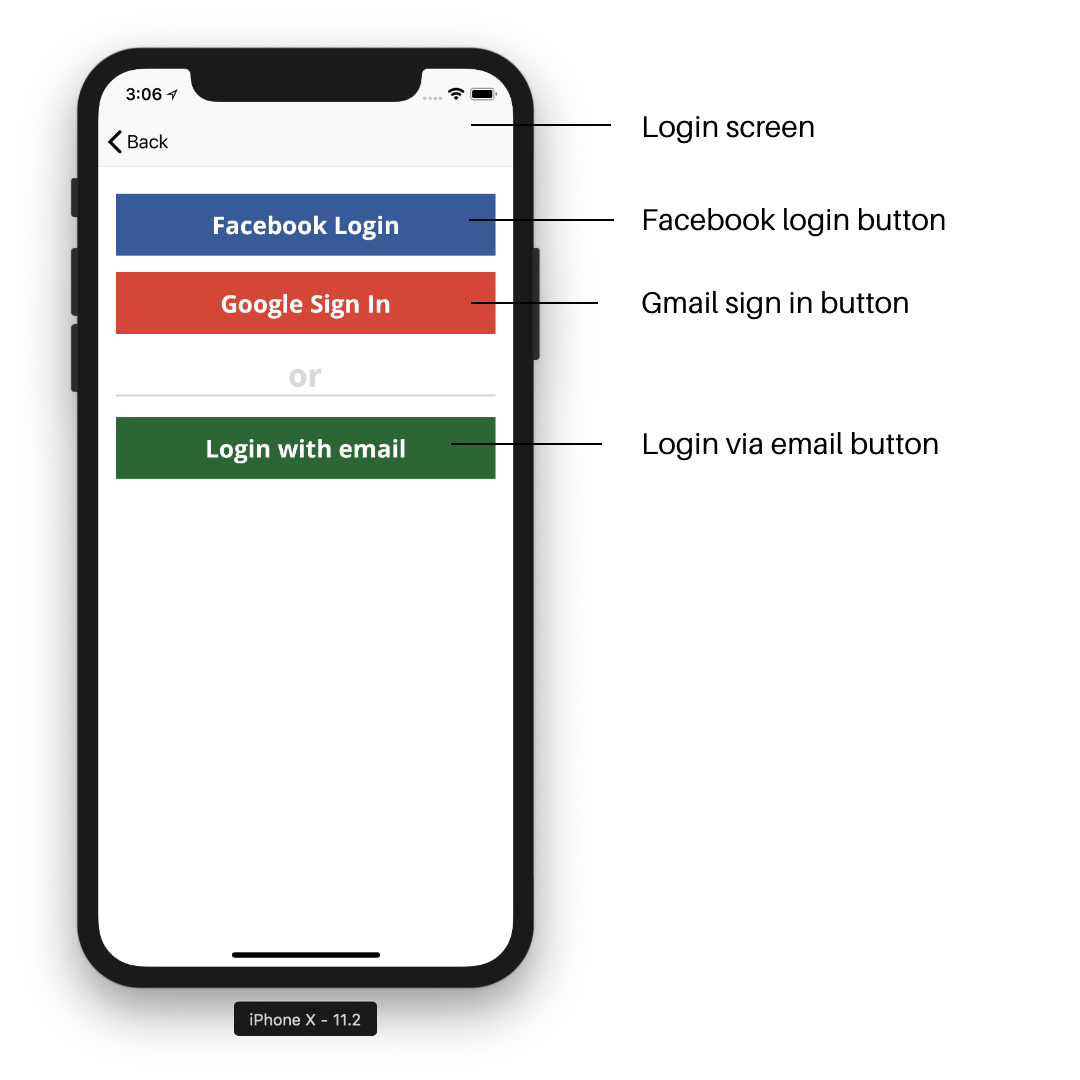
\includegraphics[width=0.5\linewidth]{figures/ch2/loginOptions.png}
            \caption{\label{fig:main_screen} Login options in the app}
    \end{figure}
    
     \textbf{1. Sign in via Social Accounts}
     
     \begin{itemize}
         \item Facebook login
         \item Gmail login
     \end{itemize}
   
     \textbf{2. Sign in via Email} \\
     
     Presently, that you have chosen to log in by means of email alternative, it takes you to that screen which requires your qualifications to enter the application, by entering the correct certifications and squeezing log in catch, you enters the application. The screen has appeared in the fig 2.4.
     
     \begin{figure}[H]
            \centering
            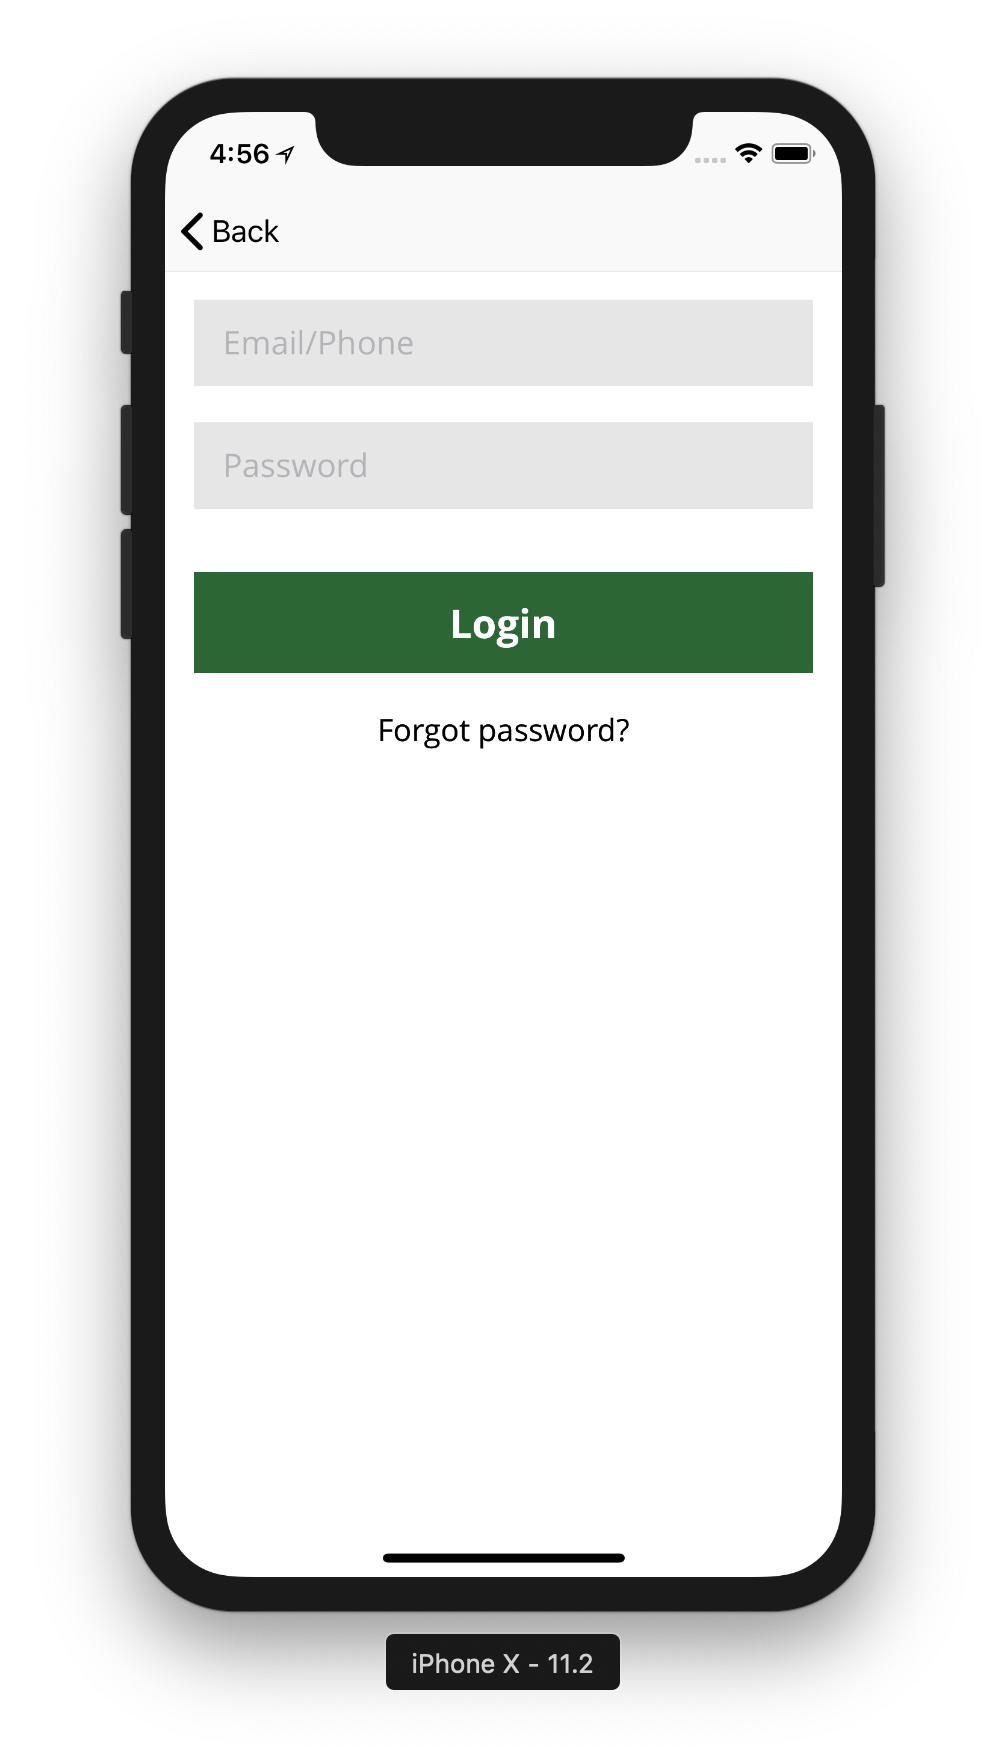
\includegraphics[width=0.5\linewidth]{figures/ch2/login_email.png}
            \caption{\label{fig:main_screen} Log in via email}
    \end{figure}
    
    
    \item \textbf{Home} \\
    \\
    Up until this point, you have took during the time spent downloading and marking in the application. Presently, it's the ideal opportunity for you to realize what's inside the application for you. \\
    
    When you log in in the application, straight way, you arrives on the home screen which fundamentally has everything what you have to utilize the application.
    
    The page that you see here is shown in the fig 2.5.
    
    \begin{figure}[H]
            \centering
            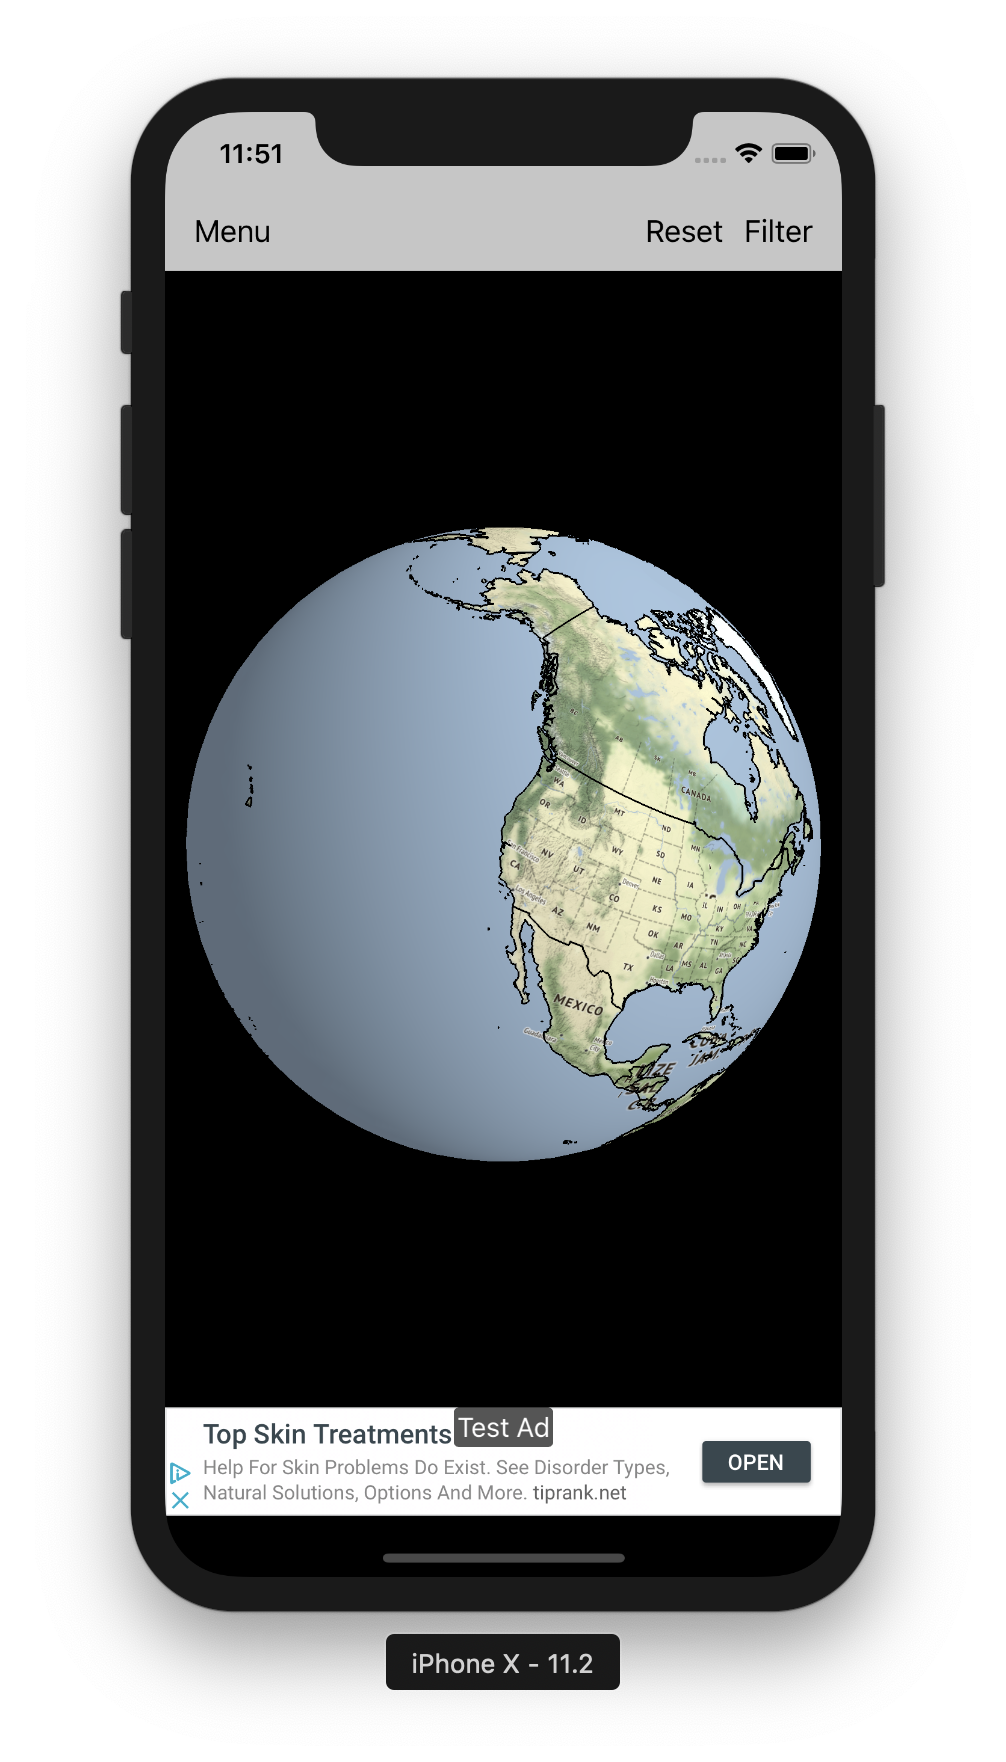
\includegraphics[width=0.5\linewidth]{figures/ch2/home.png}
            \caption{\label{fig:home_screen} Home page - landing page after log in}
    \end{figure}
    
    In this home page, you have various options for navigating in the app.\\
    
    \item \textbf{Slide out menu} \\
    
    In the event that you select \textbf{Menu}, slide out menu shows up with a few highlights. Here is the thing to note, slide out menu has been utilized to give the application an extremely pleasant look in light of keeping the ease of use while exploring in the application.
    It has been shown in the fig 2.6.
    
     \begin{figure}[H]
            \centering
            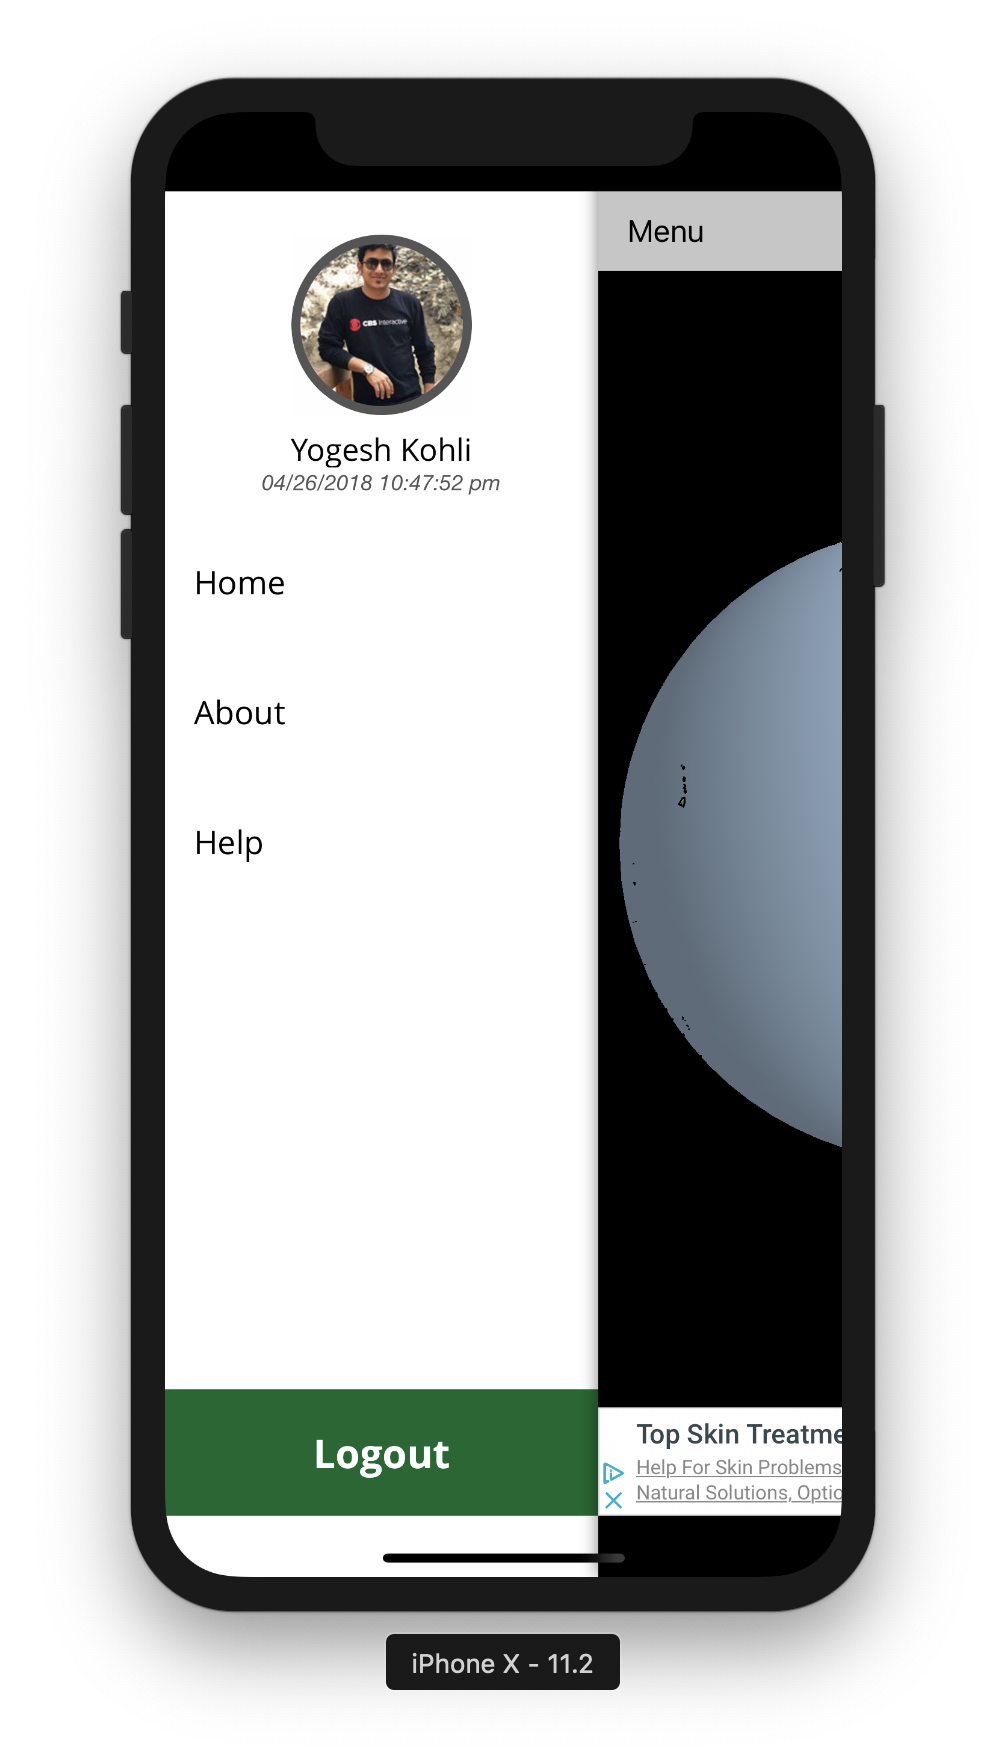
\includegraphics[width=0.5\linewidth]{figures/ch2/side_menu_1.png}
            \caption{\label{fig:slide_out_menu} Slide out menu after selecting menu option on Home screen}
    \end{figure}
    
    
   \item \textbf{Filter screens} \\
    
    Presently, in the event that you would have chosen \textbf{Filter} option on Home screen, it would have taken you to a filter screen where you have a few choices of sifting the \gls{ndvi} information that you need to see on globe/map. The figure with the number 2.7 has demonstrated as follows.
    
    \begin{figure}[H]
            \centering
            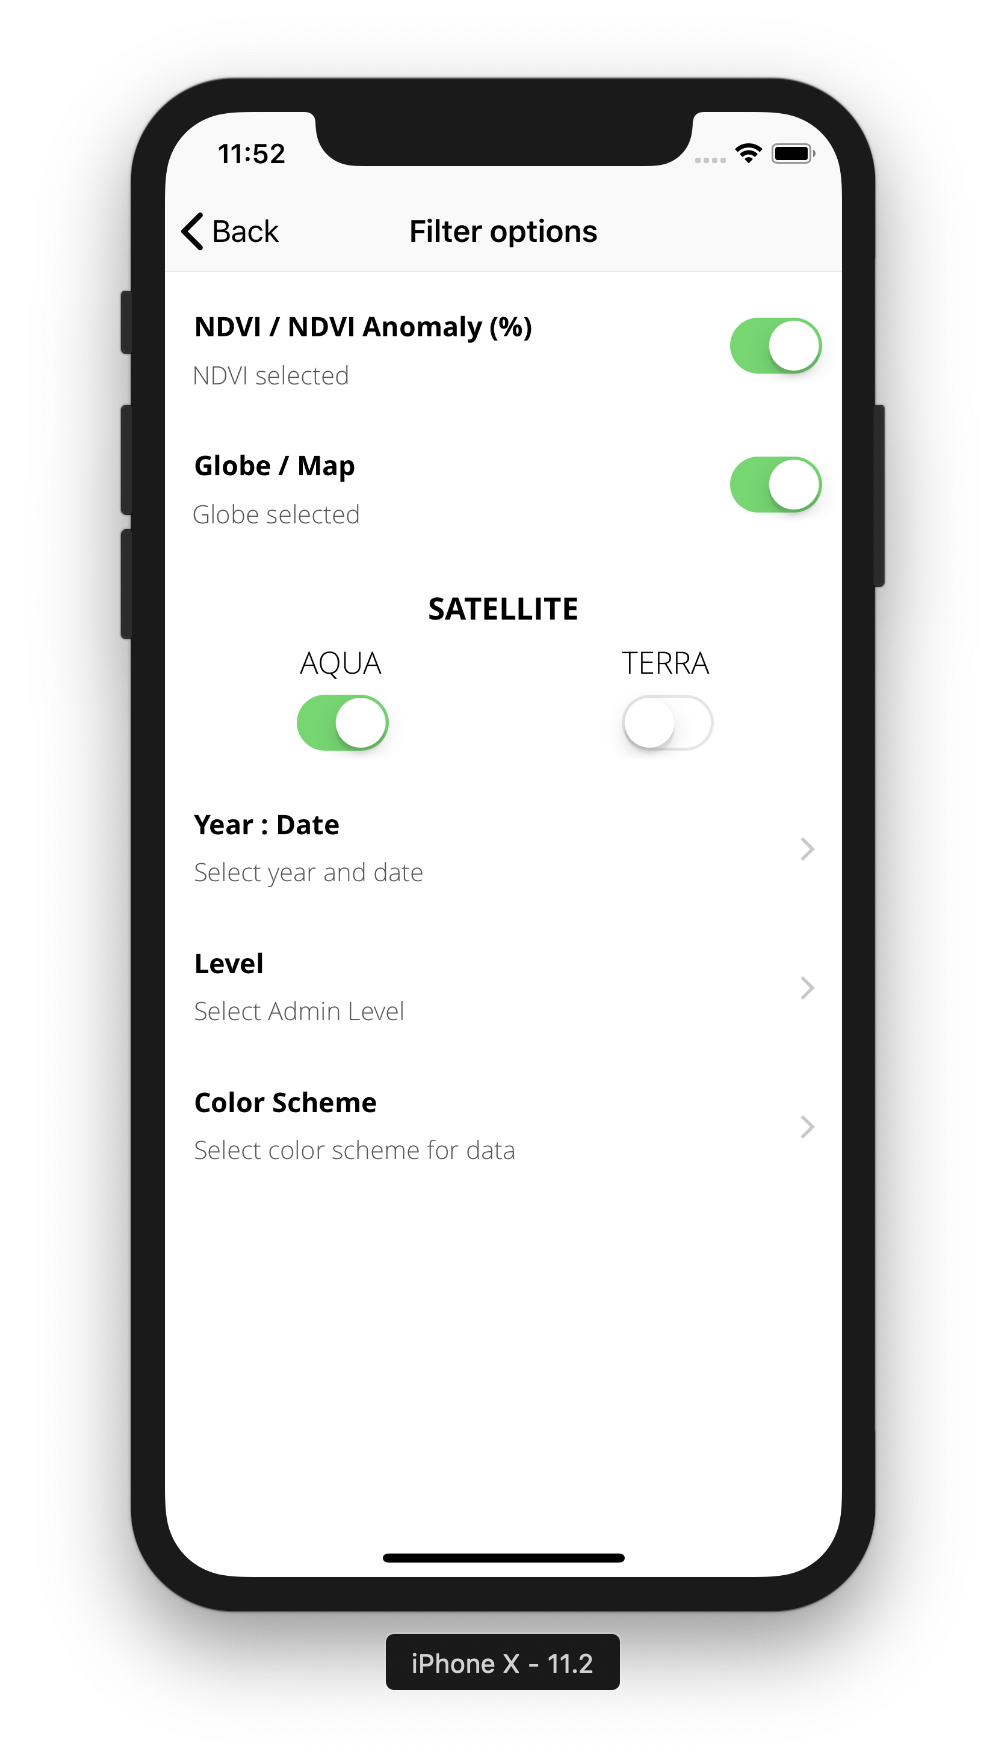
\includegraphics[width=0.5\linewidth]{figures/ch2/filter_screen.png}
            \caption{\label{fig:filter_screen} Filter screen after selecting filter option on Home screen}
    \end{figure}
    
    Now, you have various ways to filter your data.
    
    \newpage
    
    \begin{itemize}
        \item \textbf{Year list}
        
        Year - Date wise click on filter screen takes you here, shown in fig 2.8.
        
         \begin{figure}[H]
            \centering
            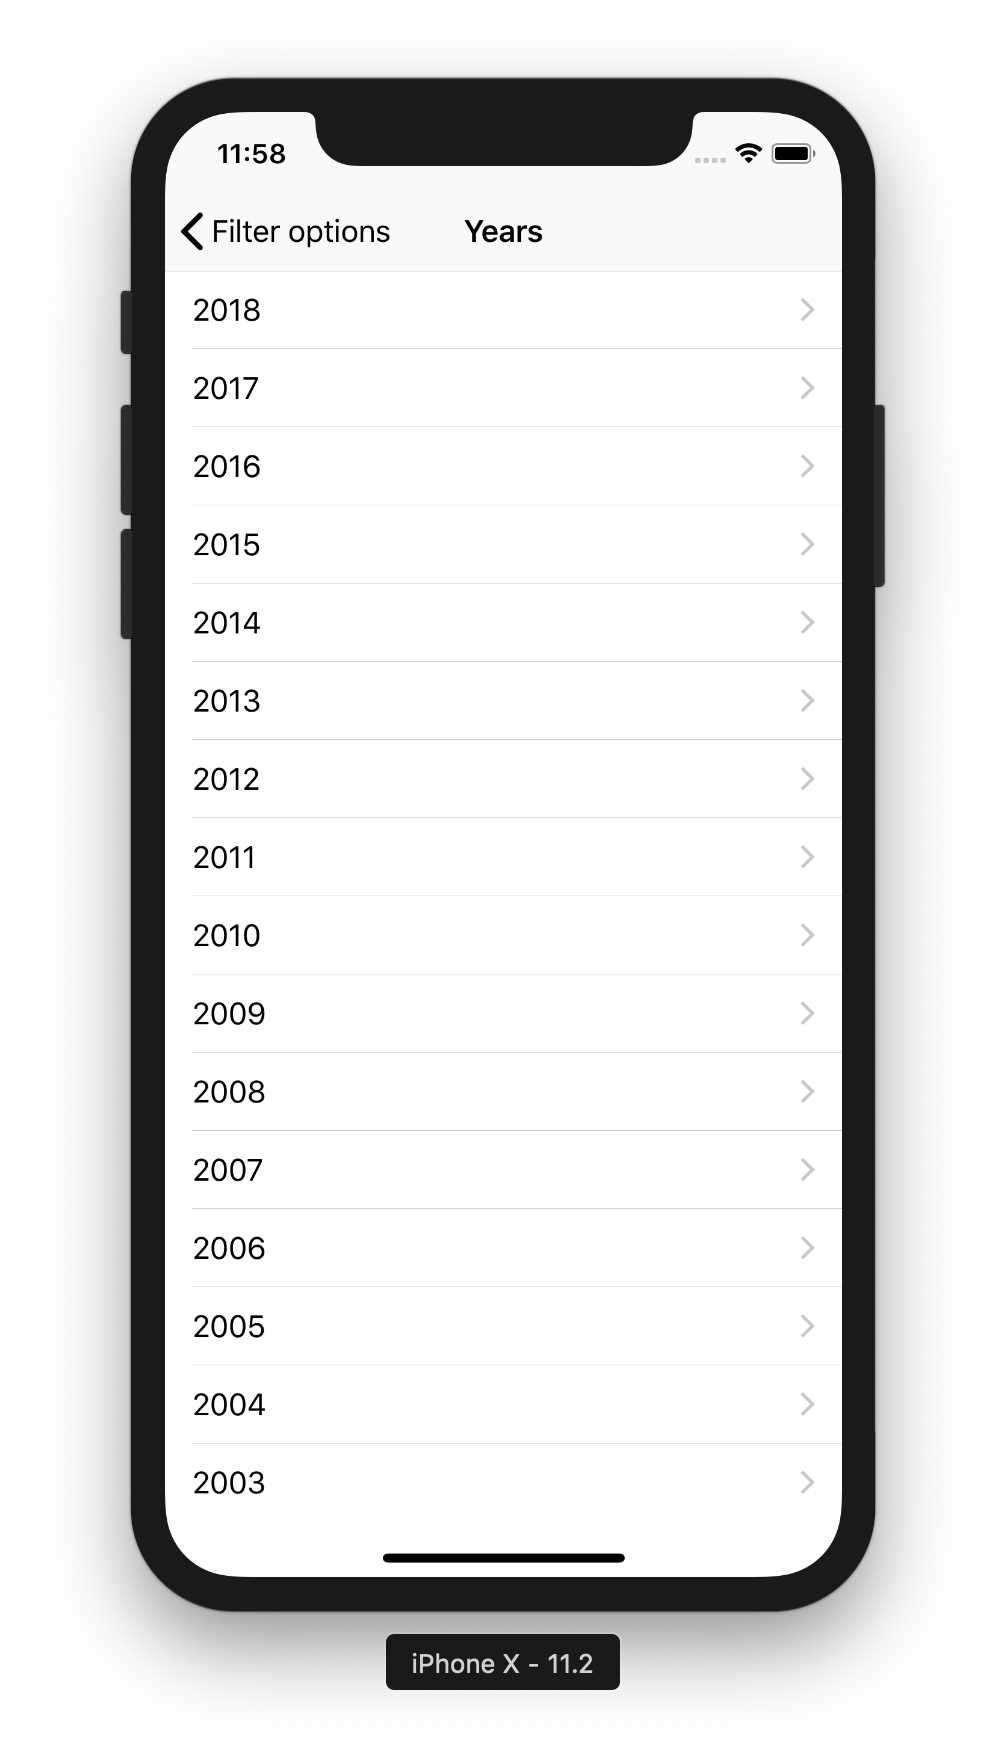
\includegraphics[width=0.5\linewidth]{figures/ch2/year_list.png}
            \caption{\label{fig:years_list_screen} Filter - Year list screen}
    \end{figure}
    
    \newpage
        
        \item \textbf{Admin level list}
        
        Admin Level click takes you here, shown in fig 2.9.
        
         \begin{figure}[H]
            \centering
            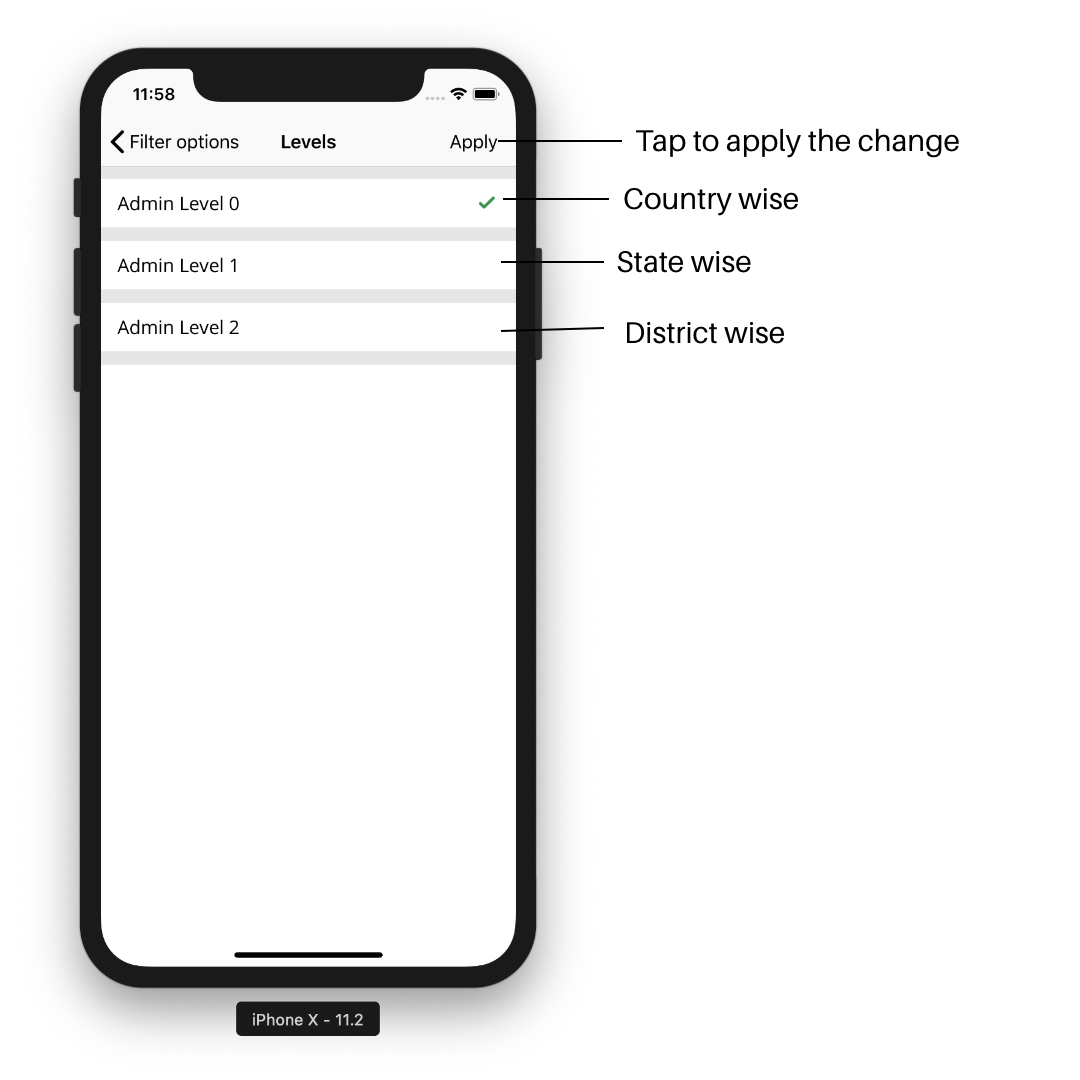
\includegraphics[width=0.5\linewidth]{figures/ch2/level_list.png}
            \caption{\label{fig:level_list_screen} Filter - Admin level list screen}
        \end{figure}
    
    \newpage
    
     \item \textbf{Color scheme list}
     
     Color scheme click takes you here, shown in fig 3.0.
        
        \begin{figure}[H]
            \centering
            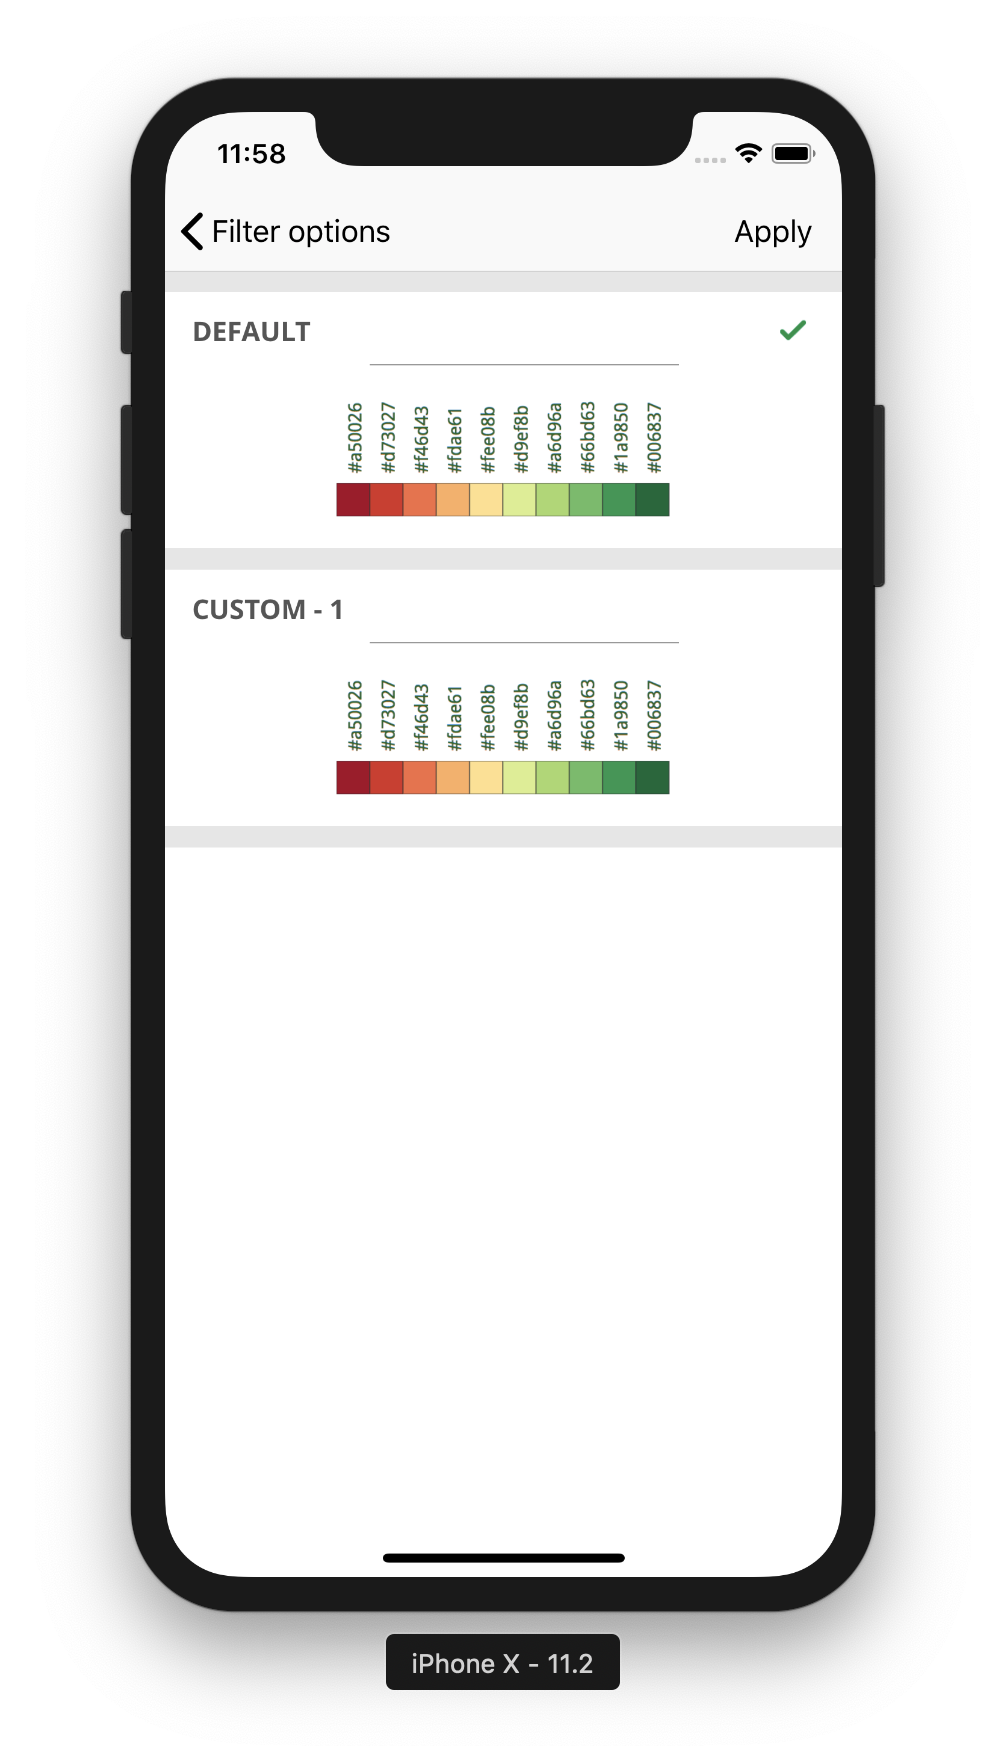
\includegraphics[width=0.5\linewidth]{figures/ch2/color_scheme.png}
            \caption{\label{fig:level_list_screen} Filter - Color palette  options screen}
        \end{figure}
        
    \end{itemize}

\end{itemize}



